\chapter{Stand der Forschung}
\section{Gold Standard}
% Was definiert einen guten Gold Standard?
Öffentliche Datensätze, welche Daten in Textform beinhalten, sind in verschiedenen Kategorien verfügbar\footnote{\url{https://medium.com/@dataturks/rare-text-classification-open-datasets-9d340c8c508e} abgerufen am: 25.06.2019}.
Auch Datensätze, die Informationen über Menüs beinhalten, sind bereits öffentlich verfügbar\footnote{\url{https://data.world/data-society/discover-the-menu} abgerufen am: 25.06.2019}.
Deutsche Textdatensätze sind bereits weniger verbreitet wie solche in englischer Sprache\footnote{\url{http://wortschatz.uni-leipzig.de/en/download/} abgerufen am: 25.06.2019}.
Einen auf der deutschen Sprache basierender Datensatz, welcher Informationen über Menüseiten beinhaltet, konnte nicht gefunden werden.
\section{Klassifikation}
Eine Methode, um Text in verschiedene Kategorien zu klassifizieren, ist das Erstellen von Regeln.
Mit einem ausgefeilten Regelsatz kann dies bei einer geringen Anzahl verschiedener Kategorien gut funktionieren.
Das Erstellen eines solchen Regelsatzes ist zeitaufwendig und muss mit einem repräsentativen Datensatz überprüft werden.
Somit ist es ein iterativer Prozess und der Ersteller muss über Expertenwissen im Themengebiet verfügen.
Solche Regelsätze bestehen aus \glqq Wenn-Dann\grqq-Bedingungen, welche mit logischen \glqq UND\grqq{} bzw. \glqq ODER\grqq{} Operatoren verknüpft sind in Kombination mit regulären Ausdrücken.
Mit solchen Regelsätzen können hohe Scores erreicht werden, ein grosses Problem des Erstellens solcher Regelsätze ist jedoch der Zeitaufwand, denn dieser steigt linear mit der Komplexität.
Aus diesem Grund besteht ein hoher Bedarf, Daten mittels statistischer Methoden automatisiert zu klassifizieren, ohne dass ein Mensch zuerst neue Regelsätze implementieren muss.\\
An diesem Punkt kommen Machine-Learning-Algorithmen zum Zug.
Diese analysieren einen Datensatz, bei dem die Proben bereits eine Zuteilung zur jeweiligen Kategorie hinterlegt haben, und klassifiziert künftige Daten anhand dieser Analyse. \cite[p. 125-127]{jackson2007natural}
\section{No-Free-Lunch Theorem}\label{sec:nofreelunch}
Ein Theorem des bekannten Informatikers David H. Wolpert, welches sinngemäss die Aussage trifft, dass kein Klassifizierer existiert, welcher für eine Vielzahl von Klassifikationsproblemen geeignet wäre \cite[p. 1341-1390]{Wolpert1996TheLO}.
Wenngleich das No-Free-Lunch Theorem aus mathematischer Sicht korrekt ist, hat sich in der Praxis doch gezeigt, dass gewisse Klassifikation-Alogorithmen über mehrere Problemklassen hinweg gute Resultate erzielen \cite{fernandez-delgado2014}.
\section{Klassifikationsalgorithmen}\label{sec:algos}
\subsection{Lineare Modell}
Lineare Modelle basieren auf der Annahme, dass ein linearer Zusammenhang zwischen Eingangsvariablen und Ausgangsvariablen besteht.
Lineare Modelle versuchen Parameter zu einer linearen Gleichung zu finden, welche die Trainingsdatenpunkte optimal abdecken.
Das optimale Abdecken wird mit einer Loss-Funktion ermittelt.
Die Loss-Funktion berechnet den Unterschied zwischen vorhergesagtem Wert zu tatsächlichem Wert des Trainingsdatenpunktes.
Lineare Modelle verwenden Optimierungsverfahren, welche iterativ Parameter verändern, um die Werte der Loss-Funktion zu minimieren und somit die bestmögliche Parameterzusammensetzung zu ermitteln.\cite{Frick-Wuersch}
\subsubsection{Ridge Classifier}
Der Ridge Classifier ist ein linearer Klassifizierer, welcher als Loss-Funktion die \glqq Least Square\grqq{} Funktion (eine Minimierung der quadrierten Abweichungen) und als Regularisierung die L2-Norm verwendet. Die L2-Norm wird pythagoreisch aus den Vektorwerten berechnet\footnote{\url{https://machinelearningmastery.com/vector-norms-machine-learning/} abgerufen am: 13.07.2019}.
Die Kombination aus oben erwähnter Loss-Funktion und der L2-Norm wird auch \glqq Ridge Regression\grqq{} genannt, von welcher der Klassifizierer auch seine Bezeichnung erhielt\footnote{\url{https://scikit-learn.org/stable/modules/generated/sklearn.linear_model.Ridge.html} abgerufen am: 13.07.2019} \cite{scikit-learn}.
\subsubsection{PassiveAgressive Classifier}
Der PassiveAggressive Classifier ist ein Klassifizierer für grosse Datenmengen.
Er ist verwandt mit dem Perceptron Algorithmus, da er keine Lernrate benötigt.
Der Klassifizierer funktioniert grob umschrieben so, dass wenn die Klassifizierung korrekt ist, er sich passiv verhält und seine internen Gewichte nicht anpasst.
Erst bei einer falschen Klassifizierung änderen seine interne Gewichte aggressiv, so dass die Fehlklassifizierung behoben wird. \cite{crammer2006online}
\subsubsection{SGDClassifier}
Der SGDClassifier gehört zur Familie der linearen Modelle\footnote{\url{https://scikit-learn.org/stable/modules/generated/sklearn.linear_model.SGDClassifier.html} abgerufen am: 14.05.2019} \cite{scikit-learn}.\\
Der \glqq Stochastic-Gradient-Descent-Classifier\grqq{} verwendet als Optimierungsvefahren das \glqq Stochastic Gradient Descent\grqq{} Verfahren\footnote{\url{https://scikit-learn.org/stable/modules/sgd.html} abgerufen am: 14.05.2019}.
Bei diesem kommt der mathematische Gradient zum Einsatz.
Der Gradient zeigt bei der Optimierung der Parameter immer in die Richtung, in welcher der Fehler (gemessen an der Loss-Funktion) am stärksten minimiert werden kann.\\
Der stochastische/probabilistische Anteil dieses Verfahrens bedeutet, dass bei der Berechnung des Gradienten jeweils nur ein Subset des ganzen Trainingsdatensatzes verwendet wird.
Dies hat den Vorteil, dass die Trainingszeit optimiert werden kann und zugleich gute Werte erzielt werden können\cite{lecun2012efficient}.\\
In der \cref{fig:sgd} wird der Verlauf der Loss-Funktion aufgezeigt und wie der Gradient zu interpretieren ist.
\begin{figure}[H]
	\centering	
	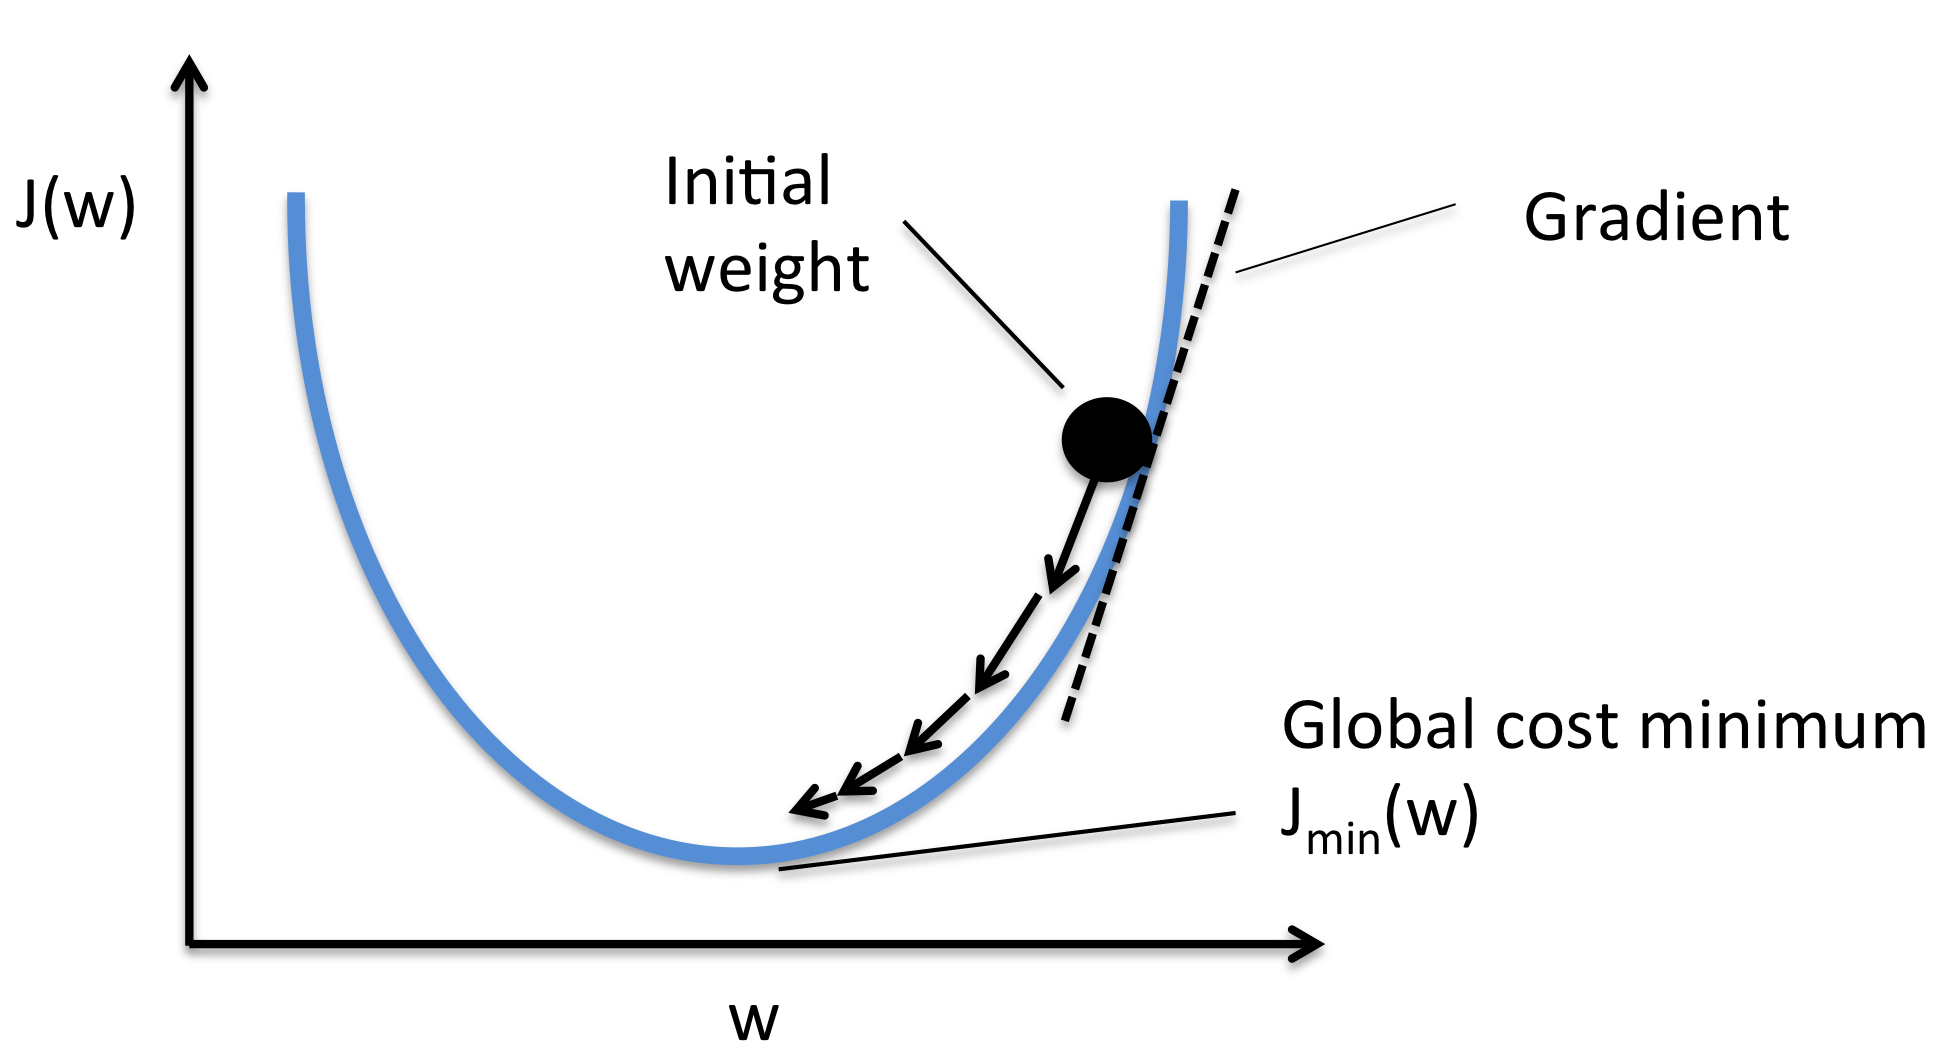
\includegraphics[width=0.7\columnwidth,keepaspectratio]{img/sgd.png}
	\caption{Visualisierung des Gradienten und der Loss-Funktion (J(w) = Loss; w = Parameteränderung)}
	\source{\url{http://rasbt.github.io/mlxtend/user_guide/general_concepts/gradient-optimization/}}
	\label{fig:sgd}
\end{figure}
\subsubsection{Perceptron}
In der \cref{fig:perceptron-grafik} ist die Darstellung eines Perceptrons ersichtlich.
Ein Perceptron ist ein Knoten, welcher allen Input-Variablen \glqq x1-x3\grqq{} eine Gewichtung(Ein Mass für die Wichtigkeit) \glqq w1-w3\grqq{} zuweist.
Die gewichteten Inputs werden dann aufsummiert.
Wenn die Summe einen bestimmten Schwellwert überschreitet, schaltet der Ausgang \glqq y\grqq{} seinen Zustand um.\\
Ein einzelnes Perceptron kann als binärer Klassifizierer verwendet werden.
Im Deep-Learning Umfeld werden mehrere Perceptronen miteinander verbunden, um ein neuronales Netzwerk zu erstellen\footnote{\url{https://towardsdatascience.com/perceptron-the-artificial-neuron-4d8c70d5cc8d} abgerufen am: 05.08.2019}.
\begin{figure}[H]
	\centering	
	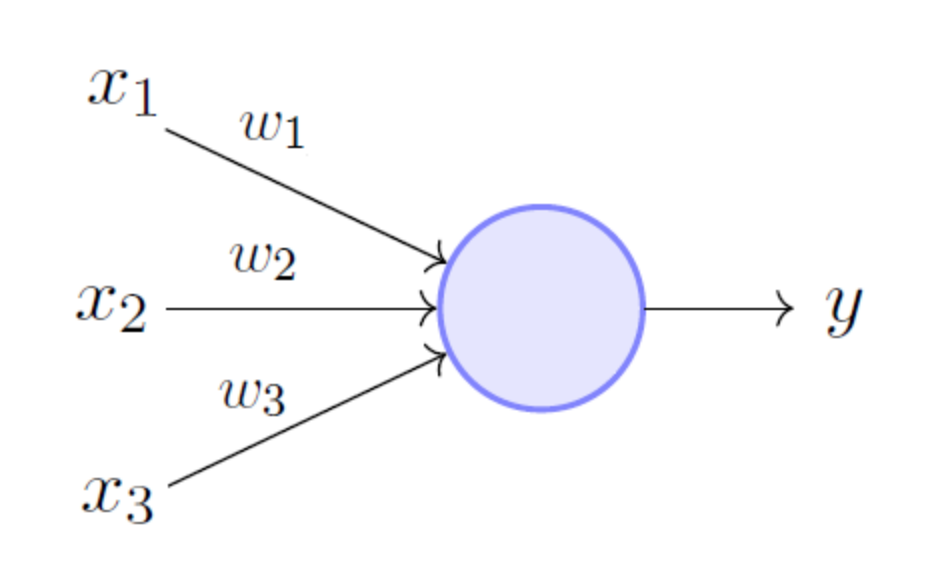
\includegraphics[width=0.6\columnwidth,keepaspectratio]{img/perceptron.png}
	\caption{Visualisierung eines Perceptrons}
	\source{\url{https://towardsdatascience.com/perceptron-the-artificial-neuron-4d8c70d5cc8d?}}
	\label{fig:perceptron-grafik}
\end{figure}
\subsection{Naive Bayes}
Naive Bayes Algorithmen sind ein Set von Supervised Learning Algorithmen, welche auf dem Theorem von Bayes basieren.\\
Das Bayes Theorem zeigt die Berechnung von bedingten Wahrscheinlichkeiten auf:
$$ P(A \mid B) = \frac{P(B \mid A) \,* P(A)}{P(B)} $$
$$ P(A) = Wahrscheinlichkeit\ von\ Ereignis\ A$$
$$ P(B) = Wahrscheinlichkeit\ von\ Ereignis\ B$$
$$ P(A \mid B) = Wahrscheinlichkeit\ von\ Ereignis\ A\ nach\ eintreffen\ von\ Ereignis\ B$$
$$ P(B \mid A) = Wahrscheinlichkeit\ von\ Ereignis\ B\ nach\ eintreffen\ von\ Ereignis\ A$$
Das Bayes Theorem kann zur Hilfe genommen werden, um bedingte Ereignisse zu berechnen\footnote{\url{https://www.crashkurs-statistik.de/der-satz-von-bayes/} abgerufen am: 16.07.2019}.
Der naive Vorsatz deutet auf die Annahme des Theorems, dass eine vollständige Unabhängigkeit zwischen allen Features herrscht.
Diese Annahme ist in der realen Welt oft nicht korrekt, trotzdem können Naive Bayes Algorithmen gute Scores erreichen und werden oft als Referenz verwendet. \cite{rennie2003tackling}
\subsubsection{Multinomial Naive Bayes}
Der Multinomial Naive Bayes Algorithmus verwendet die Annahme, dass die unabhängigen Features einer Multinomialverteilung folgen.
Für jede Klasse werden Multinomial-Parameter bestimmt.
Diese Parameter sind Vektoren, welche die Wortwahrscheinlichkeiten, dass die Wörter in den entsprechenden Klassen vertreten sind, aufzeigen.
Die Wahrscheinlichkeit, dass ein Dokument zu einer Klasse gehört, wird mit dem Produkt aller Wortwahrscheinlichkeiten aus den Vektoren bestimmt, welche sich im Dokument befinden. \cite{rennie2003tackling}
\subsubsection{Gaussian Naive Bayes}
Der Gaussian Naive Bayes Algorithmus verwendet die Annahme, dass die unabhängigen Features einer Normalverteilung folgen\footnote{\url{https://scikit-learn.org/stable/modules/naive_bayes.html} abgerufen am: 16.07.2019} \cite{scikit-learn}.
\subsubsection{Bernoulli Naive Bayes}
Der Bernoulli Naive Bayes Algorithmus verwendet die Annahme, dass die unabhängigen Features einer Bernoulliverteilung folgen.
Die Features werden als binäre Vektoren dargestellt.
Somit wird nur das Vorhandensein und nicht die Häufigkeit der Features appliziert.
Ebenfalls werden alle Relationen zwischen den unterschiedlichen Features mit der strikten Einhaltung der binären Bernoulliverteilung entfernt. \cite{mccallum1998comparison}
\subsubsection{Complement Naive Bayes}
Der Complement Naive Bayes Algorithmus (CNB) ist eine Abwandlung des Multinomial Naive Bayes Algorithmus.
Er eignet sich für stark ungleiche Datensets und verwendet für das Setzen der internen Gewichte die Komplemente der einzelnen Klassen.
Das heisst, um die Gewichte für die Klasse A zu setzen, werden alle Klassen ausser A für die Berechnung der Gewichte verwendet. \cite{rennie2003tackling}
\subsection{DecisionTree}\label{sec:trees}
Der DecisionTree-Algorithmus baut schrittweise eine Baumstruktur von Entscheidungszweigen auf, um eine Klassifizierungsaufgabe zu meistern.
DecisionTrees versuchen eine komplexe Aufgabe in Teilprobleme zu zerlegen und diese mit einfachen Entscheidungen zu bewältigen.
DecisionTree-Strukturen können verbessert werden, indem die Tiefe der Äste oder die Anzahl der Äste angepasst wird.
Bei stetiger Erhöhung der Tiefe oder der Anzahl der Äste steigt auch die Zeitkomplexität der DecisionTrees. \cite{safavian1991survey}
\subsection{Ensemble-Learning}
Ensemble-Learning ist ein Zusammenschluss von mehreren unterschiedlichen Klassifizierern, welche mit einem Voting-Verfahren eine schlussendliche Klassifizierung durchführen.
Ensemble-Learning basiert auf der Annahme, dass mehrere Algorithmen im Plenum eine bessere Aussage liefern können als ein Algorithmus alleine. \cite{freund1999short}
\subsubsection{RandomForestClassifier}
RandomForest gehört ebenfalls zur Familie der Ensemble-Learner\footnote{\url{https://scikit-learn.org/stable/modules/generated/sklearn.ensemble.RandomForestClassifier.html} abgerufen am: 14.05.2019}.
RandomForest ist eine Zusammensetzung von mehreren unterschiedlichen DecisionTrees (siehe \cref{sec:trees}).\\
RandomForest verwendet nun eine Vielzahl von DecisionTrees, die alle unterschiedliche Tiefen oder Anzahl Äste besitzen.
Dadurch können Entscheidungsausreisser aufgefangen und durch den Mehrheitsentscheid gedämpft werden. \cite{liaw2002classification}
\subsubsection{AdaBoostClassifier}
Bei vielen Ensemble-Verfahren werden alle Klassifizierer parallel trainiert und geben ihr Votum gleichzeitig ab.
Adaboost verwendet jedoch die Methode des \glqq Boosting\grqq{}, welche Ähnlichkeit mit der Theorie der genetischen Algorithmen hat\footnote{\url{https://scikit-learn.org/stable/modules/ensemble.html} abgerufen am: 14.05.2019}.
Bei Adaboost wird ein Algorithmus trainiert, validiert und als Ursprung verwendet. Alle zusätzlichen Algorithmen, welche das finale Voting durchführen, werden vom Ursprungsalgorithmus abgeleitet.
Es werden jedoch bei den Abkömmlingen die internen Parameter schrittweise verbessert und versucht die Fehler des \glqq Vater-Algorithmus\grqq{} zu vermeiden.
AdaBoost kann verbessert werden, indem die Anzahl von Vererbungsschritten angepasst wird. \cite{freund1999short}
\subsection{Nearest Neighbor Modelle}
Der Nearest Neigbhor (NN) Algorithmus ist einer der simpelsten Entscheidungsprozesse für Klassifikationen.
Beim NN Algorithmus werden Datenpunkte entsprechend ihren nächsten Nachbarn klassifiziert. \cite{cover1967nearest}
Dieses Verhalten ist in der \cref{fig:knn} für unterschiedliche Schwellwerte der Anzahl Nachbarn ersichtlich.
\begin{figure}[H]
	\centering	
	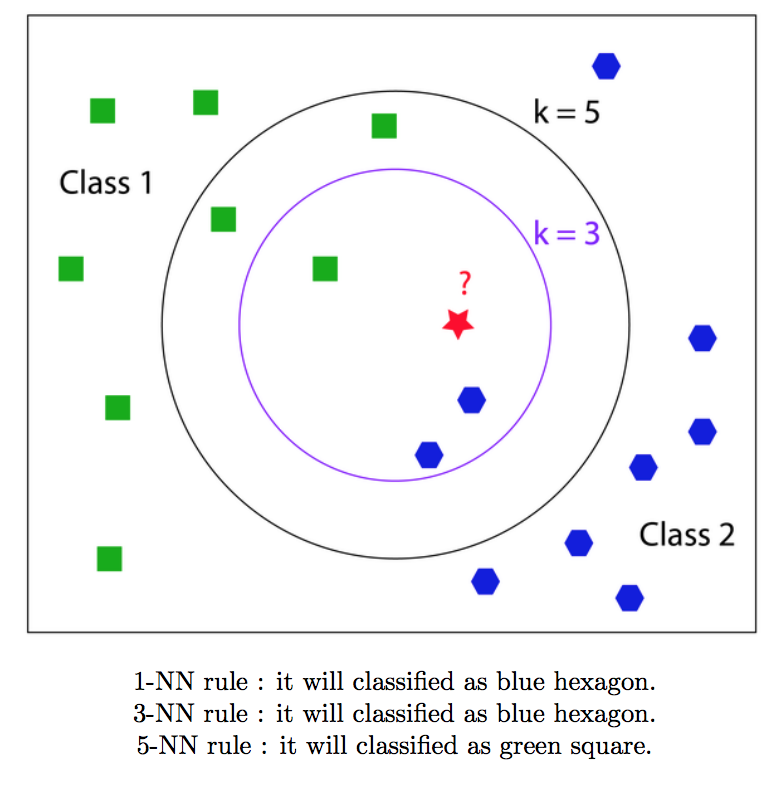
\includegraphics[width=0.7\columnwidth,keepaspectratio]{img/knn.png}
	\caption{Darstellung einer simplen K-Nearest Neighbor Prozedur}
	\source{\cite{cover1967nearest}}
	\label{fig:knn}
\end{figure}
\subsubsection{K-Nearest-Neighbor}
Der KNN Algorithmus funktioniert nach dem gleichen Prinzip wie der NN Algorithmus.
Ein Unterschied ist, dass eine spezifische Anzahl von Nachbarn mit der Kennzahl K definiert wird.
Alle K-nächsten Datenpunkten klassifizieren den gesuchten Datenpunkt mit einem Mehrheitsentscheid.
Dies ist in der \cref{fig:knn} für K=3 und K=5 ersichtlich.
K kann frei gewählt werden und dient hervorragend als Parameter für ein Hyperparametertuning (siehe \cref{sec:hyp}). \cite{cover1967nearest}
\subsubsection{Nearest Centroid}
Der Nearest Centroid Algorithmus basiert auf dem Prinzip des NN Algorithmus.
Zuerst werden die Schwerpunkte aller Klassen berechnet, indem alle zur Klasse zugewiesenen Datenpunkte miteinbezogen werden.
Danach wird der zu klassifizierende Datenpunkt der Klasse mit der kleinsten Differenz von Datenpunkt zu Schwerpunkt der Klasse zugewiesen.
Somit wird für den Nearest Centroid Algorithmus nicht der Mehrheitsentscheid der nächsten Nachbarn zur Klassifikation verwendet, sondern die Distanzen zu den Klassenschwerpunkten\footnote{\url{https://scikit-learn.org/stable/modules/neighbors.html} abgerufen am: 14.05.2019}. \cite{scikit-learn}
Dieses Verhalten ist in \cref{fig:centroid} ersichtlich.
Die schwarzen Datenpunkte markieren jeweils den Schwerpunkt der entsprechenden Klasse und die Abgrenzung der einzelnen Klassen ist mit gestrichenen, schwarzen Linien dargestellt.
\begin{figure}[H]
	\centering	
	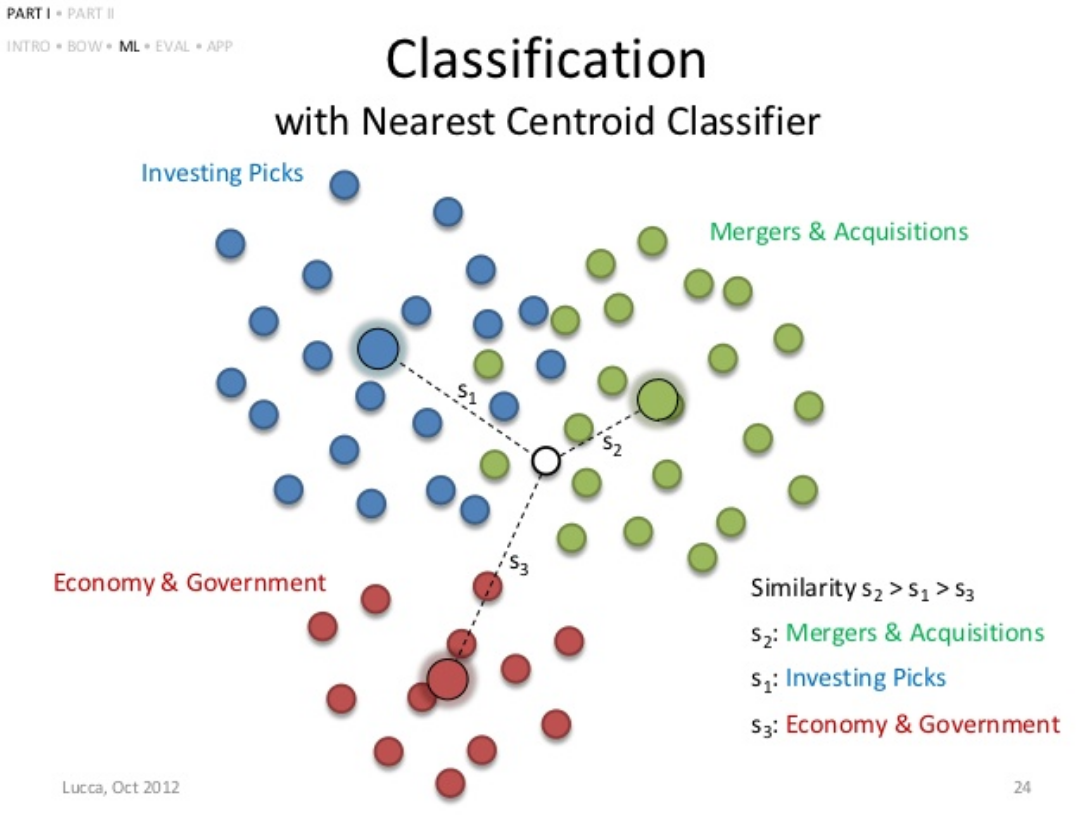
\includegraphics[width=0.7\columnwidth,keepaspectratio]{img/centroid.png}
	\caption{Darstellung einer simplen Nearest Centroid Prozedur}
	\source{\url{https://www.researchgate.net/figure/Abbildung-410-Illustration-des-Nearest-Centroid-Verfahrens-mit-den-Gruppen-soft_fig4_267488030}}
	\label{fig:centroid}
\end{figure}
\subsection{Support Vector Machine Modelle}
SVM-Classifier (Support Vector Machine) erzielen gute Resultate bei der Klassifizierung von Textdateien.
Ein Vorteil von SVM ist, dass ihre Lernrate unabhängig von der Dimension der Features ist. \cite{joachims1998text}
Dies wird erreicht, da SVM nicht auf die ganzen Features angewiesen ist.
Zwischen den unterschiedlichen Klassen werden Hyperebenen gelegt, welche das Ziel haben, die Abstände zu den einzelnen Klassen zu maximieren.
In der \cref{fig:svm} ist eine solche Hyperebene ersichtlich.
Die Features, welche am nächsten zu den Hyperebenen liegen, werden Support Vektoren genannt.
Der Algorithmus kann nach der Trennung der Klassen nun die Position von neuen Features bestimmen und somit eine Schätzung einer geeigneten Klasse vornehmen. \cite{tong2001support}
\begin{figure}[H]
	\centering	
	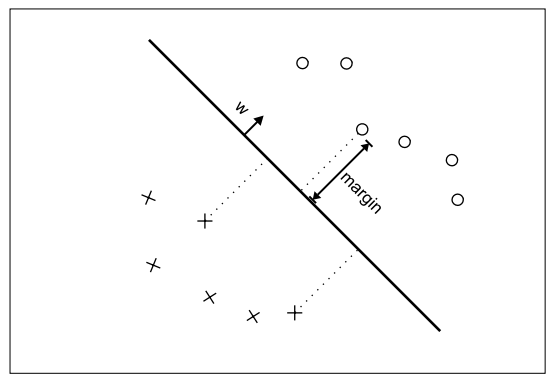
\includegraphics[width=0.7\columnwidth,keepaspectratio]{img/svm.png}
	\caption{Darstellung einer simplen Support Vector Machine}
	\source{\cite{tong2001support}}
	\label{fig:svm}
\end{figure}
\section{Hyperparametertuning}\label{sec:hyp}
Parameter, welche nicht selbstständig vom Machine-Learning Modell angepasst werden können, werden Hyperparameter genannt.
Diese Hyperparameter definieren das Verhalten von den Modellen.
Die geeignetsten Hyperparameter können mit einer ausführlichen Suche gefunden werden, was als Hyperparametertuning bezeichnet wird\footnote{\url{https://scikit-learn.org/stable/modules/grid_search.html} abgerufen am: 14.05.2019}. \cite{scikit-learn}